\section{Lược khảo tài liệu} % Section 2
\subsection{Tổng hợp các tài liệu, nghiên cứu trước liên quan}

\subsubsection{Nghiên cứu về nhận diện biểu cảm khuôn mặt (FER)}
Nhận diện biểu cảm khuôn mặt (Facial Expression Recognition - FER) là một lĩnh vực trọng điểm trong thị giác máy tính. Từ đầu những năm 2000, các phương pháp truyền thống như LBP, HOG, hoặc SIFT kết hợp với SVM từng chiếm ưu thế. Tuy nhiên, chúng không hiệu quả trong điều kiện ánh sáng thay đổi hoặc góc nhìn khác nhau. Từ năm 2014, học sâu - đặc biệt là CNN - đã nâng cao độ chính xác mô hình FER. Các kiến trúc như VGGNet, ResNet, InceptionNet đạt độ chính xác 70--75\% trên FER-2013 nhưng yêu cầu tài nguyên tính toán lớn. [3]

\subsubsection{Ảnh hưởng của điều kiện ánh sáng yếu}
Zhang et al. (2019), Wang et al. (2022) đã chứng minh rằng ảnh thiếu sáng làm giảm hiệu quả của mô hình FER. GAN-based như EnlightenGAN hoặc RetinexNet giúp cải thiện nhưng đòi hỏi GPU mạnh, không phù hợp với thiết bị thực tế như điện thoại hoặc camera nhúng. [[2], [8]]

\subsubsection{Các kỹ thuật tiền xử lý ảnh tăng cường sáng}
\textbf{Gamma Correction}: điều chỉnh độ sáng theo hàm \(I_{out} = I_{in}^\gamma\). Với \(\gamma < 1\), ảnh được làm sáng. [9]\par
\textbf{CLAHE}: nâng cao độ tương phản cục bộ, phù hợp ảnh có vùng sáng tối không đều. Wang et al. (2021) dùng CLAHE trước FER đạt cải thiện đáng kể. [4]

\subsubsection{Mô hình học sâu nhẹ: MobileNetV3}
MobileNetV3 (Howard et al., 2019) là CNN nhẹ, tối ưu cho thiết bị di động, gồm kỹ thuật như depthwise separable convolution, squeeze-and-excitation và NAS. MobileNetV3-Small có \~2.5M tham số, cân bằng tốt giữa độ chính xác và hiệu suất, chưa được nghiên cứu sâu trong FER ánh sáng yếu. [[5], [6], [7]]

\begin{figure}[H]
    \centering
    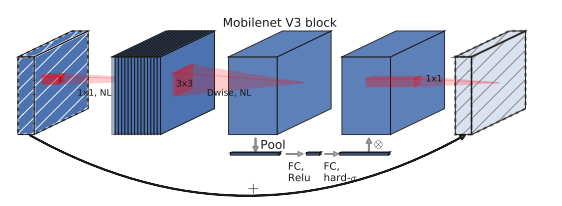
\includegraphics[width=0.7\textwidth]{img/mobinetv3.png} % Đường dẫn tương đối
    \caption{Mô hình MobileNetV3.}
    \label{fig:emotion_distribution}
\end{figure}


\subsection{Cơ sở lý thuyết của nghiên cứu}
Nghiên cứu kết hợp tiền xử lý ảnh thích ứng theo điều kiện ánh sáng và mô hình CNN nhẹ - MobileNetV3 để tăng hiệu suất FER trong điều kiện ánh sáng yếu.

\subsubsection{Tiền xử lý ảnh trong điều kiện ánh sáng yếu}
\textbf{Gamma Correction [9]}: hàm phi tuyến giúp làm sáng ảnh thiếu sáng. Ying et al. (2017) chỉ ra rằng \(\gamma\) phù hợp có thể nâng cao chất lượng ảnh mà không gây nhiễu.\par
\textbf{CLAHE [4]}: phân tích cục bộ từng vùng ảnh, cải thiện chi tiết biểu cảm ở vùng mắt, miệng (Zhu et al., 2018).\par
\textbf{Tính thích ứng [10]}: thuật toán tự động phân tích histogram và độ sáng trung bình để chọn phương pháp phù hợp (Chen et al., 2021).

\subsubsection{Nhận diện biểu cảm bằng mô hình CNN nhẹ – MobileNetV3}
MobileNetV3-Small [5] (Howard et al., 2019): \~2.5 triệu tham số, thích hợp cho thiết bị nhúng. Nghiên cứu dùng mô hình này để fine-tune phân loại 7 biểu cảm.\par
\textbf{Kỹ thuật chính}: Depthwise Separable Convolution (Howard et al., 2017) [5], SE Module (Hu et al., 2018) [11], Hard-Swish Activation.

\subsubsection{Pipeline đề xuất trong nghiên cứu}

Dựa trên hai thành phần lý thuyết đã trình bày, nghiên cứu đề xuất pipeline xử lý gồm 3 giai đoạn chính như trong Bảng~\ref{tab:pipeline}:

\begin{table}[H]
\centering
\caption{Pipeline đề xuất trong nghiên cứu}
\label{tab:pipeline}
\begin{tabular}{|p{4cm}|p{10cm}|}
\hline
\textbf{Giai đoạn} & \textbf{Nội dung} \\
\hline
\textbf{Tiền xử lý ảnh} &
\begin{itemize}[leftmargin=*]
    \item Chuyển ảnh sang ảnh grayscale.
    \item Tính độ sáng trung bình $\mu$.
    \item Nếu $\mu < T_1$: áp dụng gamma correction với $\gamma \in [0.4, 0.5]$.
    \item Nếu $T_1 < \mu < T_2$: áp dụng CLAHE.
    \item Nếu $\mu > T_2$: giữ nguyên hoặc áp dụng contrast stretching nhẹ.
\end{itemize} \\
\hline
\textbf{Học biểu cảm} &
\begin{itemize}[leftmargin=*]
    \item Ảnh sau tiền xử lý được đưa vào mô hình MobileNetV3-Small.
    \item Mô hình được fine-tune để phân loại 7 biểu cảm: vui, buồn, giận, sợ, bất ngờ, ghê tởm, trung tính.
\end{itemize} \\
\hline
\textbf{Đánh giá mô hình} &
\begin{itemize}[leftmargin=*]
    \item Thực hiện trên tập test có và không áp dụng tăng cường ảnh.
    \item Sử dụng các chỉ số đánh giá:
    \begin{itemize}
        \item Accuracy
        \item Precision / Recall
        \item F1-score
        \item Confusion Matrix
    \end{itemize}
    \item So sánh với baseline không áp dụng tăng cường để đánh giá hiệu quả thực sự.
\end{itemize} \\
\hline
\end{tabular}
\end{table}

Bảng~\ref{tab:pipeline} mô tả chi tiết \textbf{pipeline xử lý} được đề xuất trong nghiên cứu, bao gồm ba giai đoạn chính: \textit{tiền xử lý ảnh}, \textit{học biểu cảm}, và \textit{đánh giá mô hình}. Trong giai đoạn tiền xử lý, ảnh đầu vào được chuyển sang ảnh xám và điều chỉnh độ sáng hoặc tương phản dựa trên giá trị trung bình $\mu$ của ảnh. Tùy theo mức độ sáng, các kỹ thuật như gamma correction, CLAHE hoặc contrast stretching nhẹ sẽ được áp dụng nhằm cải thiện chất lượng ảnh đầu vào.

Tiếp theo, giai đoạn học biểu cảm sử dụng mô hình \textit{MobileNetV3-Small} đã được tinh chỉnh (fine-tune) để phân loại bảy loại biểu cảm khuôn mặt phổ biến: vui, buồn, giận, sợ, bất ngờ, ghê tởm và trung tính.

Cuối cùng, mô hình được đánh giá trên tập kiểm thử với và không có áp dụng kỹ thuật tăng cường ảnh. Các chỉ số đánh giá bao gồm Accuracy, Precision, Recall, F1-score và ma trận nhầm lẫn (Confusion Matrix). Kết quả mô hình sẽ được so sánh với một mô hình baseline không áp dụng tăng cường ảnh nhằm đánh giá hiệu quả thực sự của pipeline đề xuất.


\begin{figure}[H]
    \centering
    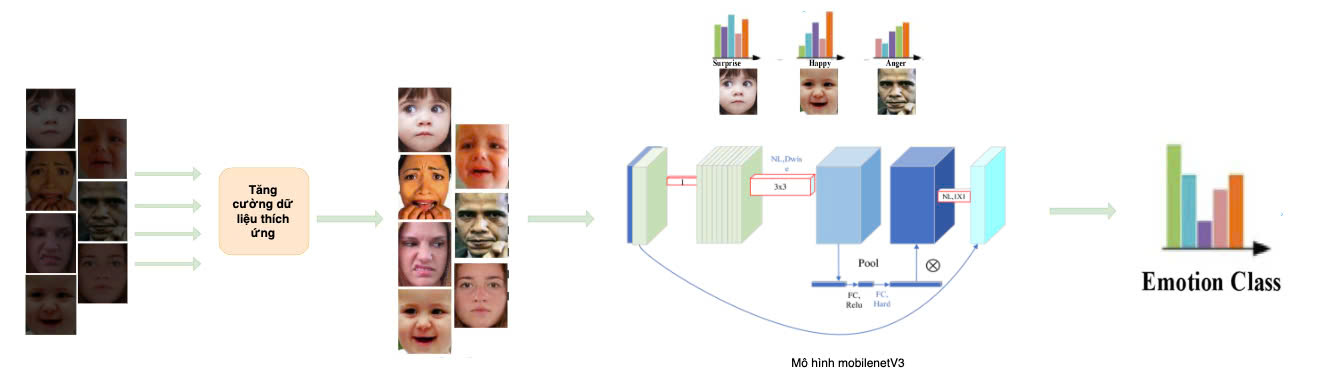
\includegraphics[width=0.85\textwidth]{img/pineline.jpg} % Đường dẫn tương đối
    \caption{Pine line đề xuất}
    \label{fig:pineline}
\end{figure}

Hình~\ref{fig:pineline} cho thấy pipeline đề xuất cho hệ thống nhận diện cảm xúc khuôn mặt. Dữ liệu ảnh đầu vào được tăng cường bằng cách điều chỉnh độ sáng nhằm cải thiện khả năng nhận diện trong các điều kiện ánh sáng khác nhau. Sau đó, ảnh được đưa vào mô hình MobileNetV3 để trích xuất đặc trưng và phân loại cảm xúc đầu ra.

\subsection{Phân tích điểm mạnh, điểm yếu của các nghiên cứu trước và hướng kế thừa}

\subsubsection{Điểm mạnh}
\begin{itemize}
    \item Mô hình học sâu giúp tăng độ chính xác FER (Mollahosseini et al., 2016) [3].
    \item MobileNetV3 hiệu quả, tiết kiệm tài nguyên (Howard et al., 2019) [[5], [6]].
    \item CLAHE giúp tăng sáng hiệu quả, đơn giản (Wang et al., 2020) [4].
\end{itemize}

\subsubsection{Hạn chế}
\begin{itemize}
    \item Chưa chú trọng ánh sáng yếu trong FER (Barsoum et al., 2016) [[3], [8]].
    \item Pipeline thiếu bước tăng cường ảnh (Zhou et al., 2021) [12].
    \item Dùng GAN tăng sáng gây tốn tài nguyên (Chen et al., 2020) [2].
\end{itemize}

\subsubsection{Hướng kế thừa và phát triển}
\begin{itemize}
    \item Chọn MobileNetV3-Small làm backbone (Howard et al., 2019) [5].
    \item Thiết kế pipeline có bước xử lý ảnh thích ứng đầu vào. [10]
    \item Mô phỏng tập FER-2013 thiếu sáng để kiểm thử.
    \item Ưu tiên tăng sáng đơn giản thay vì GAN.
\end{itemize}

% Chương 2.4 - Cơ sở lý thuyết của thuật toán tăng cường dữ liệu thích ứng
\subsection{Cơ sở lý thuyết của thuật toán tăng cường dữ liệu thích ứng} % 2.4

\subsubsection{Lý do phát triển thuật toán} % 2.4.1
Trong bài toán nhận diện biểu cảm khuôn mặt (FER -- Facial Expression Recognition) dưới điều kiện ánh sáng yếu, hình ảnh khuôn mặt thường bị suy giảm chất lượng nghiêm trọng do hiện tượng thiếu sáng toàn cục hoặc cục bộ. Điều này dẫn đến hiện tượng mất chi tiết, đặc biệt ở các vùng chứa đặc trưng biểu cảm quan trọng như mắt, miệng, nếp nhăn. Kết quả là mô hình học sâu, vốn phụ thuộc vào độ tương phản và cấu trúc cục bộ, sẽ khó khăn trong việc nhận dạng chính xác. [[10], [12]]

Các kỹ thuật tăng cường dữ liệu truyền thống như histogram equalization hoặc gamma correction thường được áp dụng đồng loạt cho toàn bộ dữ liệu huấn luyện. Tuy nhiên, cách tiếp cận này bỏ qua tính biến thiên về mức sáng của từng ảnh đầu vào. Cụ thể:
\begin{itemize}[]
    \item Với ảnh quá tối, tăng sáng quá mức dễ làm mất chi tiết do bão hòa điểm ảnh.
    \item Với ảnh sáng vừa đủ, tăng cường không cần thiết có thể làm biến dạng đặc trưng tự nhiên, dẫn đến suy giảm hiệu quả học.
\end{itemize}

Do đó, nghiên cứu này đề xuất một thuật toán tăng cường dữ liệu thích ứng, có khả năng phân tích đặc trưng ánh sáng riêng của từng ảnh, từ đó lựa chọn kỹ thuật xử lý phù hợp, đơn giản nhưng hiệu quả và phù hợp để huấn luyện với mô hình nhẹ như MobileNetV3-Small.

\subsubsection{Các thành phần lý thuyết chính} % 2.4.2
\subsubsection*{(a) Phân tích độ sáng của ảnh [9]}

Để xác định ảnh đầu vào có cần tăng cường hay không, và nếu cần thì sử dụng phương pháp nào, cần phân tích một số đặc trưng cơ bản về độ sáng:


\begin{itemize}[]
    \item \textbf{Độ sáng trung bình (mean intensity)}: Được tính trên ảnh chuyển sang thang xám (grayscale) hoặc kênh Y (luminance) trong không gian YUV.
    
    \[ \mu = \frac{1}{H \times W} \sum_{i=1}^{H} \sum_{j=1}^{W} I(i,j) \]
    
    \item \textbf{Độ lệch chuẩn (standard deviation)}: Đánh giá mức độ phân tán sáng tối, cho biết ảnh có sáng đồng đều hay có vùng sáng -- vùng tối xen kẽ.
    \item \textbf{Histogram phân bố pixel}: Dùng để xác định ảnh có độ tương phản thấp (hẹp histogram) hoặc bị lệch về vùng tối.
\end{itemize}

\subsubsection*{(b) Các kỹ thuật tăng cường ánh sáng được sử dụng [[9], [12]]}
\begin{itemize}[]
    \item \textbf{Gamma Correction:}
    \[ I_{\text{out}} = I_{\text{in}}^{\gamma} \]
    \begin{itemize}[]
        \item $\gamma < 1$: ảnh được làm sáng lên.
        \item $\gamma > 1$: ảnh bị làm tối hơn.
    \end{itemize}
    Việc chọn giá trị $\gamma$ được tính toán dựa trên giá trị độ sáng trung bình $\mu$ của ảnh.

    \item \textbf{Histogram Equalization (HE)}:
    Phân bố lại giá trị pixel để làm tăng độ tương phản tổng thể. Phù hợp khi histogram bị tập trung ở vùng tối (low dynamic range). Tuy nhiên, dễ gây nhiễu ở ảnh có noise.

    \item \textbf{Contrast Stretching:}
    Kéo dãn mức độ sáng từ dải cường độ cũ về dải chuẩn 0--255:
    \[ I_{\text{out}} = \frac{I_{\text{in}} - I_{\min}}{I_{\max} - I_{\min}} \times 255 \]
    

      \begin{figure}[H]
    \centering
    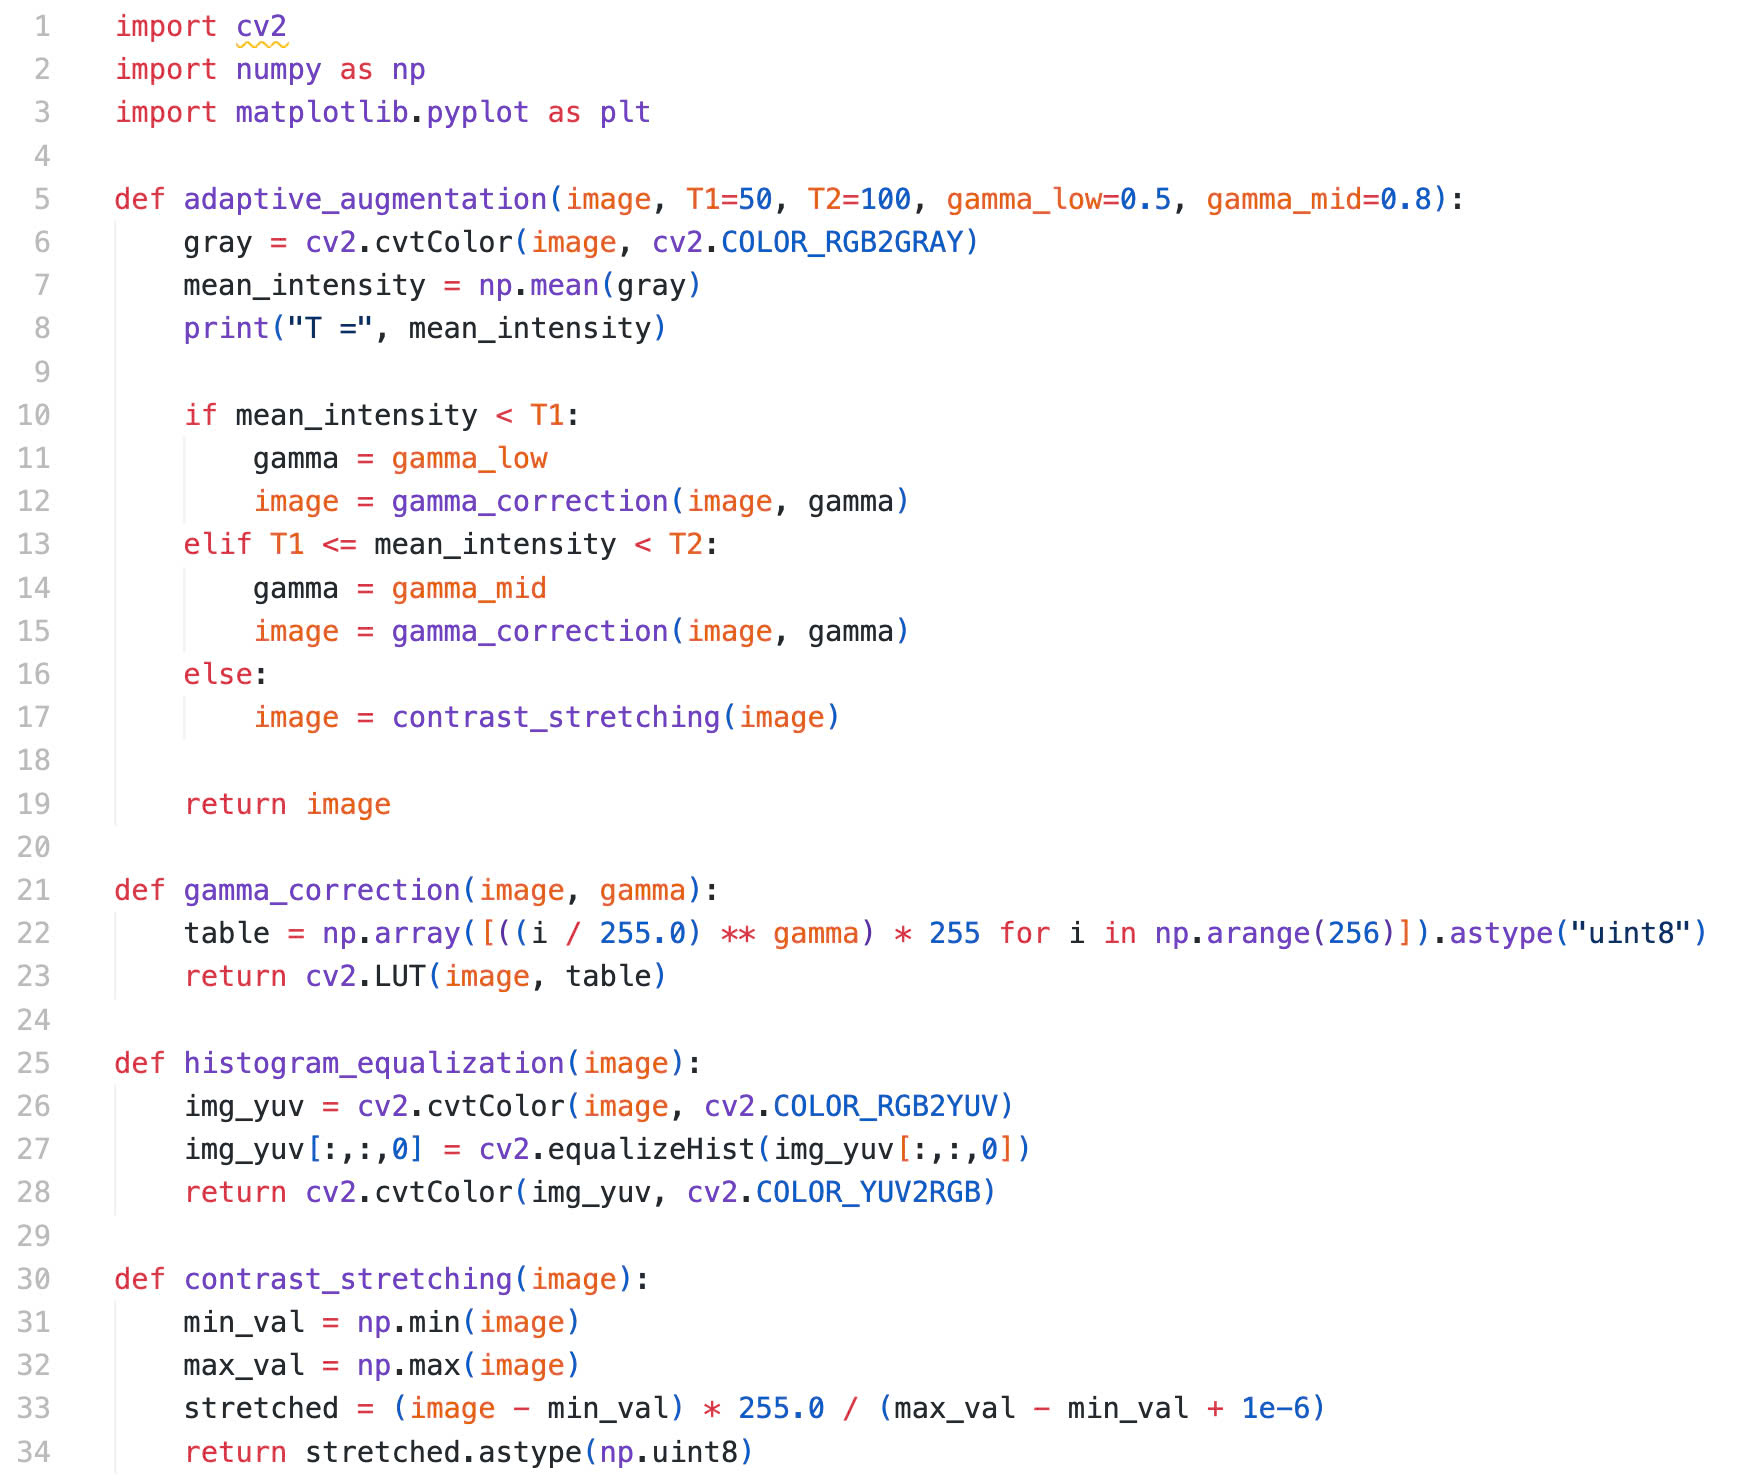
\includegraphics[width=0.7\textwidth]{img/thuatToan_01.jpg} % Đường dẫn tương đối
    \label{fig:emotion_distribution}
\end{figure}
  \begin{figure}[H]
    \centering
    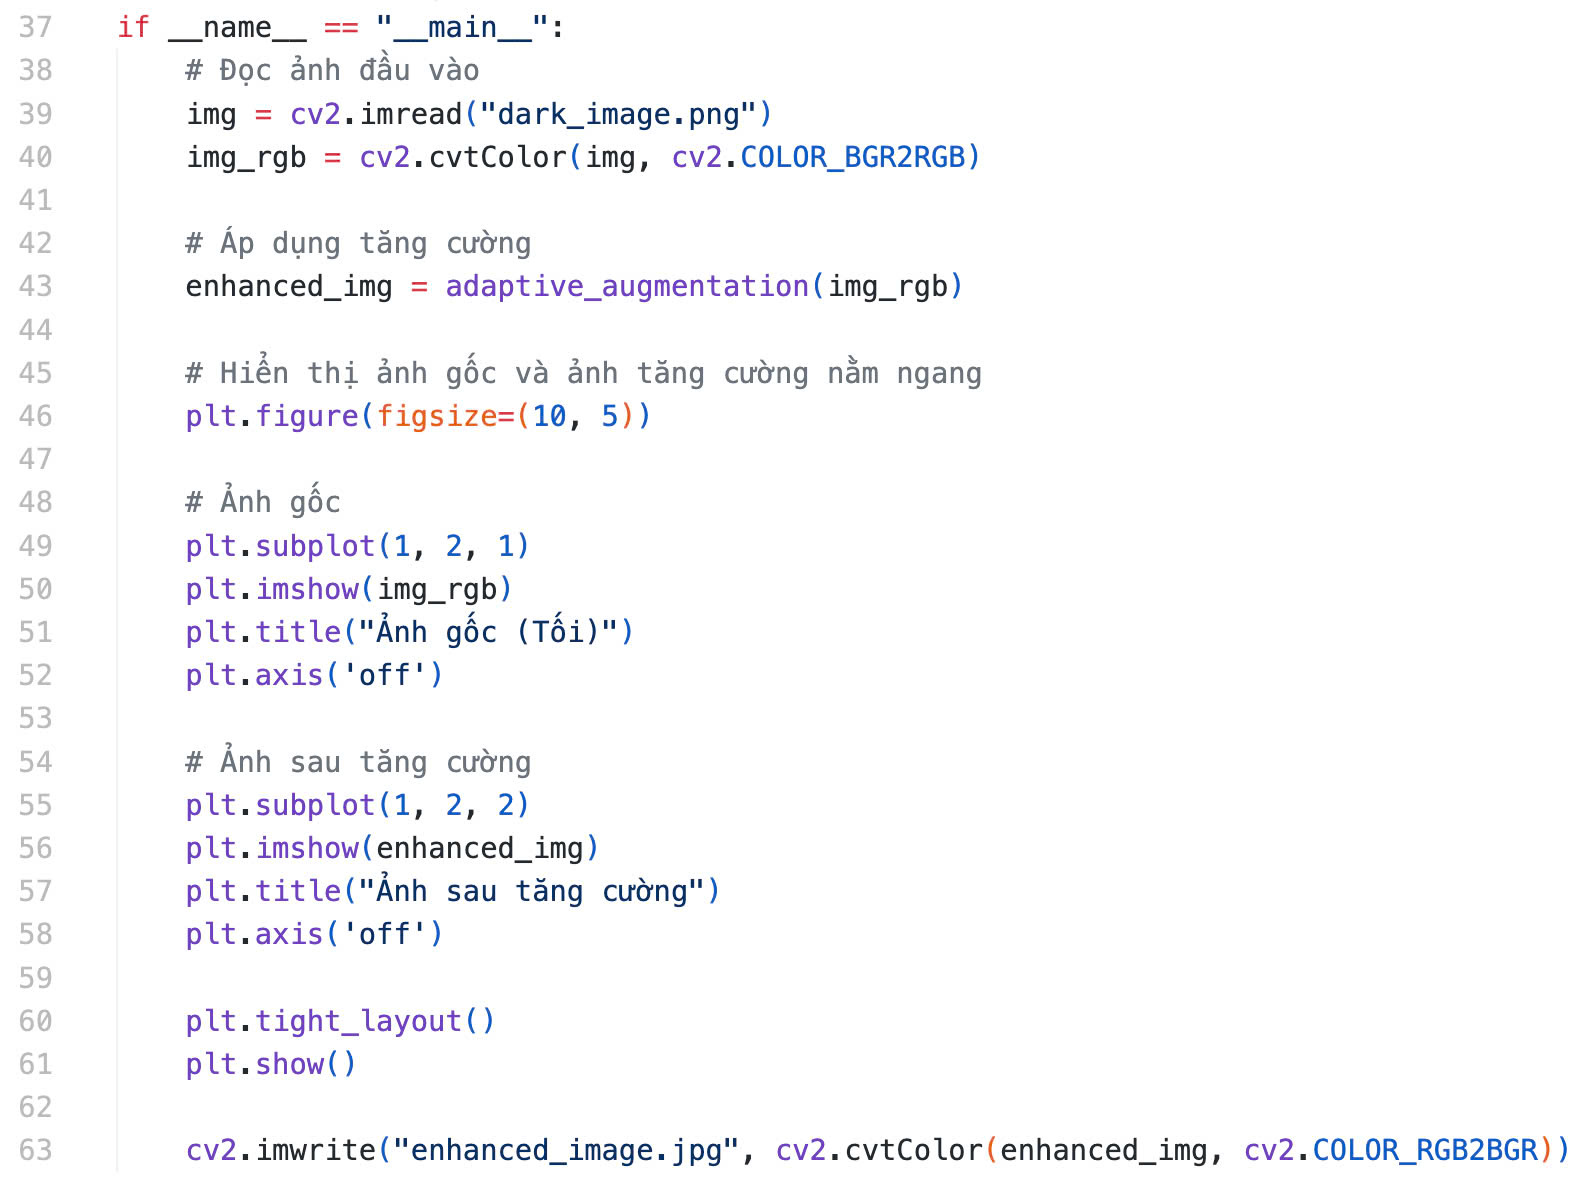
\includegraphics[width=0.7\textwidth]{img/thuatToan_02.jpg} % Đường dẫn tương đối
    \caption{Code minh họa}
    \label{fig:emotion_distribution}
\end{figure}


    \begin{figure}[H]
    \centering
    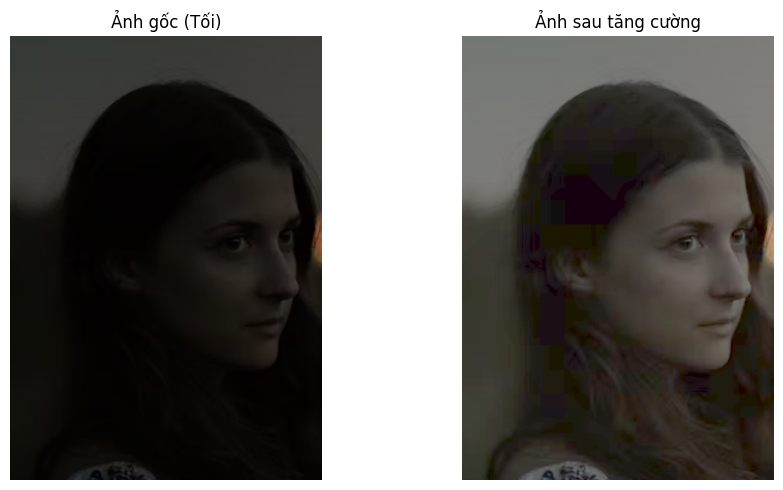
\includegraphics[width=0.7\textwidth]{img/anhsautangcuong.png} % Đường dẫn tương đối
    \caption{Ảnh trước và sau khi tăng cường}
    \label{fig:emotion_distribution}
\end{figure}
\end{itemize}

\subsubsection*{(c) Tính thích ứng của thuật toán [10]}
Thuật toán sẽ:
\begin{itemize}[]
    \item Tính toán độ sáng trung bình ($\mu$) và độ lệch chuẩn ($\sigma$) của từng ảnh đầu vào.
    \item Dựa vào hai ngưỡng xác định trước $T_1$ và $T_2$, phân loại mức độ ánh sáng:
    \begin{itemize}[]
        \item $\mu < T_1$ (ảnh rất tối): áp dụng gamma nhỏ (0.3--0.5).
        \item $T_1 \le \mu < T_2$ (tối vừa): áp dụng gamma nhẹ (0.7--0.9) hoặc HE.
        \item $\mu \ge T_2$ (sáng đủ): không tăng cường hoặc chỉ contrast stretching nhẹ.
    \end{itemize}
\end{itemize}
Cách tiếp cận này giúp mỗi ảnh được tăng cường đúng mức, tránh làm hỏng đặc trưng gốc hoặc gây dư sáng.

\subsubsection{Nguồn cảm hứng và các nghiên cứu liên quan} % 2.4.3

Retinex-based methods (Fu et al., 2020) đề xuất kỹ thuật phân tách ảnh thành hai thành phần: phản xạ và ánh sáng chiếu vào, sau đó tái cấu trúc lại ảnh với độ sáng cải thiện. Phương pháp này cho kết quả nâng cao rõ rệt nhưng đòi hỏi thuật toán phức tạp và tài nguyên tính toán lớn, do đó khó triển khai trên các thiết bị nhúng. [2]

GAN-based methods như EnlightenGAN (Jiang et al., 2019) sử dụng mạng sinh ảnh để tạo lại phiên bản ảnh có ánh sáng tốt hơn từ ảnh thiếu sáng ban đầu. Mặc dù đem lại chất lượng thị giác cao, nhưng các mô hình GAN thường yêu cầu GPU mạnh và thời gian xử lý lâu, khiến chúng không phù hợp với các ứng dụng thời gian thực trên thiết bị di động. [2]

Adaptive Augmentation trong học sâu (Zhang et al., 2021) nhấn mạnh tầm quan trọng của việc sử dụng đặc trưng đầu vào để quyết định chiến lược tăng cường dữ liệu phù hợp, thay vì áp dụng cố định một kỹ thuật như truyền thống. Điều này giúp mô hình học sâu đạt hiệu quả tốt hơn trong môi trường đầu vào đa dạng.

Từ các nghiên cứu trên, thuật toán của nhóm đề xuất kế thừa ý tưởng \textit{adaptive preprocessing}, nhưng được đơn giản hóa để giảm chi phí tính toán và đảm bảo tính linh hoạt, phù hợp với các mô hình nhẹ như MobileNetV3. [12]
